% --------------------------------------------------------------------
% Preamble
% --------------------------------------------------------------------
\documentclass[paper=a4, fontsize=11pt,twoside]{scrartcl}    % KOMA

\usepackage[a4paper,pdftex]{geometry}    % A4paper margins
\setlength{\oddsidemargin}{5mm}            % Remove 'twosided' indentation
\setlength{\evensidemargin}{5mm}

\usepackage[english]{babel}
\usepackage[protrusion=true,expansion=true]{microtype}    
\usepackage{amsmath,amsfonts,amsthm,amssymb}
\usepackage{listings}
\usepackage{graphicx}
\usepackage{setspace}
\usepackage{hyperref}
\usepackage{ragged2e}
\usepackage{tabto}
\usepackage{afterpage}
\usepackage[usenames, dvipsnames]{color}
\usepackage{titlesec}
\usepackage{lipsum}
\usepackage{tipa}
\usepackage{amsthm}
\usepackage{relsize}
\usepackage{color}
\usepackage{chngcntr}
\usepackage{textcomp}
\usepackage[binary-units=true]{siunitx}
\numberwithin{table}{section}
\numberwithin{figure}{section}


% --------------------------------------------------------------------
% Definitions
% --------------------------------------------------------------------
\newcommand{\HRule}[1]{\rule{\linewidth}{#1}}     % Horizontal rule

\makeatletter                            % Title
\def\printtitle{%                        
    {\centering \@title\par}}
\makeatother                                    

\makeatletter                            % Author
\def\printauthor{%                    
    {\large \@author}}                
\makeatother       

\newcommand\blankpage{%
    \null
    \thispagestyle{empty}%
    \addtocounter{page}{-1}%
    \newpage}                     

\definecolor{mygray}{gray}{0.6}

\titleformat{\section}
{\normalfont\huge\bfseries}
{\thesection\hskip 12pt\textcolor{mygray}{\textdoublepipe}\hskip 20pt}
{0pt}
{}

\titlespacing*{\section}{0pt}{18pt}{13pt}

\newtheorem{ddef}{Definition}[section]


\definecolor{mygreen}{rgb}{0,0.6,0}
\definecolor{mygray}{rgb}{0.5,0.5,0.5}
\definecolor{mymauve}{rgb}{0.58,0,0.82}

\lstset{
  backgroundcolor=\color{white},   % choose the background color
  basicstyle=\footnotesize,        % size of fonts used for the code
  breaklines=true,                 % automatic line breaking only at whitespace
  captionpos=b,                    % sets the caption-position to bottom
  commentstyle=\color{mygreen},    % comment style
  escapeinside={\%*}{*)},          % if you want to add LaTeX within your code
  keywordstyle=\color{blue},       % keyword style
  stringstyle=\color{mymauve},     % string literal style
}


% --------------------------------------------------------------------
% Metadata
% --------------------------------------------------------------------

\title{
	\begin{flushright}
		\LARGE{\textit{Scott Williams}}
	\end{flushright}
	~\\[2.0cm]			
	\normalsize \textsc{Computer Science Part II Project Dissertation}\\[2.0cm]     % Subtitle
    \HRule{0.5pt} \\                        % Upper rule
    \LARGE \textbf{\uppercase{Steganographic file systems within video files}}    % Title
    \HRule{2pt} \\[30pt]        % Lower rule + 0.5cm spacing
    \normalsize Christ's College\\[5pt]University of Cambridge\\[25pt]           
    \normalsize \today            % Todays date
}

\begin{document}
\renewcommand{\thelstlisting}{\thesection.\arabic{lstlisting}}
% ------------------------------------------------------------------------------
% Maketitle
% ------------------------------------------------------------------------------
\thispagestyle{empty}        % Remove page numbering on this page

\printtitle                    % Print the title data as defined above
\vfill
\printauthor                % Print the author data as defined above
\afterpage{\blankpage}
\newpage
% ------------------------------------------------------------------------------
% Begin document
% ------------------------------------------------------------------------------
\setcounter{page}{1}        % Set page numbering to begin on this page
\pagenumbering{roman}
\section*{Performa}
\NumTabs{3}
\textsc{Name}: \tab{Scott Williams}\\
\textsc{College}: \tab{Christ's}\\
\textsc{Project Title}: \tab{Steganographic file systems within video files}\\
\textsc{Examination}: \tab{Part II of the Computer Science Tripos}\\
\textsc{Year}: \tab{2015}\\
\textsc{Word Count}: \tab{12,000}\\
\textsc{Project Originator}: \tab{Scott Williams}\\
\textsc{Project Supervisor}: \tab{Daniel Thomas}\\

\subsection*{Original Aims of the Project}
% 350 words per day...
To investigate appropriate steganographic embedding methods for video and to develop a practical steganographic software package to enable the embedding of arbitrary data within video files via a file system interface. Raw AVI video files should be supported and a variety of steganograhpic embedding algorithms should be available. Basic file system commands should work within the presented logical volume and embedding should occur with no perceivable impact on video quality.

\subsection*{Work Completed}
A complete software package has been developed enabling the embedding of arbitrary files within many video formats (including MP4 and AVI) via a file system interface. A total of 9 steganographic embedding algorithms are supported, along with encryption and plausible deniability functionality. Basic file system operations work as expected within the mounted volume and the embedding process can operate without any perceivable impact on video quality. Performance of the system is adequate for general use allowing high definition media content to be played directly out of the embedded volume.

\subsection*{Special Difficulties}
None.

\pagebreak
\section*{Declaration of Originality}
~\\[5pt]
I, Scott Williams of Christ's College, being a candidate for Part II of the Computer
Science Tripos, hereby declare that this dissertation and the work described
in it are my own work, unaided except as may be specified below, and that
the dissertation does not contain material that has already been used to any
substantial extent for a comparable purpose.

I give permission for my dissertation to be made available in the archive
area of the Laboratory's website.\\[20pt]
\textit{Signed:}\\[20pt]
\textit{Date:}
\clearpage

\tableofcontents
\vfill

\pagebreak
\pagenumbering{arabic} 
\section{Introduction}
Steganography is the art of hiding information in apparently innocuous objects. Whereas cryptography seeks to protect only the content of information, steganography attempts to conceal the fact that the information even exists. This allows steganographic methods to be utilised in countries where encryption is illegal for example, or within the UK where keys for identified encrypted data can be forced to be handed over.

In this project I design and implement a practical steganographic software application - \texttt{Stegasis} - which enables users to embed arbitrary files within videos via a file system interface. \texttt{Stegasis} can operate with no perceivable impact on video quality and can achieve embedding capacities of upto 200\% of the video size. A wide range of video formats are supported\footnote{Including many modern video formats such as \texttt{MP4}, \texttt{MKV}, \texttt{FLV} and \texttt{AVI}.} along with several steganographic embedding algorithms. Standard encryption algorithms can be used to further protect embedded data and plausible deniability functionality protects users even when the presence of embedded data has been confirmed.

Steganogaphic methods operating on video have had comparatively little attention compared to images and audio. As such, there are few programs currently available which allow data to be steganographically hidden within video. \texttt{Stegasis} is the first application to enable the embedding of arbitrary files within videos via a file system interface.   



\subsection{Motivation}
Digital media is ubiquitous on the Internet and high definition video content is now common place on video sharing and social networking websites. Video files of multiple gigabytes in size can reside on users devices without arousing suspicion, providing an ideal hiding place for large collections of sensitive files. Few programs are capitalising on this fact, and those that are, allow the user to embed only a singe chosen file into a small range of video formats with very low embedding capacities. As with \texttt{TrueCrypt}\footnote{A successful cryptographic program providing on-the-fly encryption and full disc encryption.}, I believe that a practical system for protecting sensitive files should present the user with a mounted logical volume allowing the use of standard file system operations to create, access and organise embedded data. Furthermore, there exist many commonly used video formats along with many more currently in development. As such, a steganographic program operating on a small number of video formats not only greatly restricts usability, it will require constant development as new video formats inevitably become more popular. Instead, a generic solution applicable to a variety of video formats is preferred.

The many recent global surveillance disclosures show that using certain technologies related to privacy can get you ``flagged" by authorities such as the \texttt{NSA} - it is no longer the case that simply encrypting data is enough to keep the owner safe.

\section{Preparation}
\subsection{Background}
In this section steganographic background material, definitions and concepts are introduced. A number of related technologies to the project are also discussed.\\

\noindent
The most important property of any steganographic system is undetectability, that is, it should be impossible to differentiate between ordinary and steganographically modified objects. This requirement is famously formulated within Simmons' prisoners' problem. 

Alice and Bob are imprisoned in separate cells and wish to formulate an escape plan. They are allowed to communicate, but all messages must pass through a warden Eve. If Eve suspects the prisoners of secretly discussing their escape plan, the communication channel will be severed and Alice and Bob thrown into solitary confinement. The prisoners attempt to utilise steganograhpy to exchange details of their plan undetected. The steganographic system is considered broken if Eve is able to detect the presence of hidden messages within the prisoners exchanges. It is assumed that Eve has a complete knowledge of the steganographic algorithm being used, with the exception of the stego key, which Alice and Bob have agreed upon beforehand. This is in parallel with Kerckhoff's principle used within cryptography. The warden can be considered to be one of three categories: \textit{passive}, \textit{active} and \textit{malicious}. A passive warden does not modify the exchanged messages in any way, whereas an active warden may modify the messages whilst maintaining their original meaning. For example an active warden may replace words with synonyms or reorder sentences. If images are being used as a transport medium then an active warden may recompress or crop the images. A malicious warden attempts to break the steganograhpic system and impersonate the prisoners in an attempt to obtain information.

This project is concerned with only the case of the \textit{passive} warden. As such, any modification of the video files once \texttt{stegasis} has embedded data within them, will most likely render the embedded file system corrupt\footnote{This unfortunately means utilising video sharing websites such as YouTube and Facebook for distribution is not possible due to them performing compression upon video upload.}.


\subsubsection{Steganographic Concepts}
A steganographic system consists of a number of individual components:
\begin{itemize}
	\item A \textit{Cover object} is the original object that the message will be embedded within.
	\item A \textit{Message} is an arbitrary length sequence of symbols. For this project we consider a message $\mathcal{M} \in \{0,1\}^{n} $ that is, a binary string.
	\item A \textit{Stego key} is a secret key used within the embedding process.
	\item A \textit{Stego object} is the result of embedding a message inside a cover object.
\end{itemize}

\begin{ddef}
\textsc{Steganographic System}\\[5pt]
Let $\mathcal{C}$ be the set of all cover objects. For a given $\textbf{c} \in \mathcal{C}$, let $\mathcal{K} _{\textbf{c}}$ denote the set of all stego keys for \textbf{c}, and the set $\mathcal{M} _{\textbf{c}}$ denote all messages that can be communicated in \textbf{c}. A steganographic system\footnote{This is specifically steganography by cover modification.}, is then formally defined as a pair of embedding and extracting functions Emb and Ext,
\begin{center}
	Emb :  $\mathcal{C} \times \mathcal{K} \times \mathcal{M} \rightarrow \mathcal{C}$\\
	Ext :  $\mathcal{C} \times \mathcal{K} \rightarrow \mathcal{M}$\\
\end{center}
satisfying,
\begin{center}
	$\forall ~\textbf{c}, \textbf{k}, \textbf{m}. ~\textbf{c} \in \mathcal{C} ~\land ~ \textbf{k} \in \mathcal{K} _{\textbf{c}} ~\land ~ \textbf{m} \in \mathcal{M} _{\textbf{c}} \Rightarrow$ Ext(Emb(\textbf{c}, \textbf{k}, \textbf{m}), \textbf{k}) = \textbf{m}	
\end{center}
\end{ddef}
\begin{ddef}
\textsc{Embedding Capacity}\\[5pt]
The \textit{Embedding Capacity} (payload) $\mathcal{P} _{\textbf{c}}$ for a given cover object \textbf{c} $\in \mathcal{C}$ is defined in bits as,
\begin{center}
	$\mathcal{P} _{\textbf{c}} = \log_{2}|\mathcal{M}(\textbf{c})| $
\end{center}
The relative embedding capacity $\mathcal{R} _{\textbf{c}}$ for a given cover object \textbf{c} $\in \mathcal{C}$ is defined as,
\begin{center}
	$\mathcal{R} _{\textbf{c}} = \dfrac{\log_{2}|\mathcal{M}(\textbf{c})|}{n} $
\end{center}
where n is the number of elements in \textbf{c}.
\end{ddef}
\noindent
For example, consider $\mathcal{C}$ to be the set of all 512 $\times$ 512 greyscale images, embedding one bit per pixel gives $\mathcal{M} = \{0,1\}^{512 \times 512}$ and $\forall ~\textbf{c} \in \mathcal{C}. ~|\mathcal{M}(\textbf{c})| = 2^{512 \times 512}$. The embedding capacity $\forall ~\textbf{c} \in \mathcal{C}$ is then $512 \times 512 \approx 33$kB as expected. In this case, $n$ is equal to the number of pixels in \textbf{c} and therefore the relative embedding capacity is equal to 1 bpp (bits per pixel), again as expected.

Using the definitions above, we can define a simple expression for the embedding capacity of a video file. 
\begin{ddef}
\textsc{Embedding Capacity for video}\\[5pt]
With $\mathcal{C}$ as the set of all video files, the embedding capacity $\mathcal{V} _{\textbf{c}}$ for a given video $\textbf{c} \in \mathcal{C}$ can be expressed as,
\begin{center}
	$\mathcal{V} _{\textbf{c}} ~= \mathlarger{\mathlarger{\sum}}\limits_{f ~\in ~frames(\textbf{c})} \mathcal{P} _{f}$
\end{center}
\end{ddef}
\noindent
Note that for certain embedding algorithms, the embedding capacity can depend on both the input data and the cover object\footnote{Many algorithms operating on \texttt{JPEG} images for example will not embedded within zero valued DCT coefficients.}. However, in some cases the following expression is also valid,
\begin{center}
	$\mathcal{V} _{\textbf{c}} ~=~ |frames(\textbf{c})| \cdot \mathcal{P} _{f _{0}}$
\end{center}

\begin{ddef}
\textsc{Steganographic Capacity}\\[5pt]
The concept of Steganographic Capacity is loosely defined as the maximum number of bits that can be embedded within a given cover object without introducing statistically detectable artifacts. % <-- spelt right
\end{ddef}
\noindent
For completeness, the least significant bit (LSB) of a given number is defined as follows,
\begin{center}
	LSB($x$) = $x$ mod 2
\end{center}
% steganalysis
\subsubsection{Steganalysis}
Steganalysis is the study of detecting messages embedded using steganographic techniques; this is analogous to cryptanalysis applied to cryptography. A steganalysis attack is considered successful (that is, the steganography has been broken) if it is possible to correctly distinguish between cover and stego objects with probability better than random guessing. Note that it is not necessary to be able to read the contents of the secret message to break a steganographic system.

A trivial example of steganalysis arises when the steganalyst has access to the original cover object used within the embedding procedure. By computing the difference between the stego and cover objects, the steganalyst can immediately detect the presence of a hidden message. This attack identifies a number of important points to consider when developing a practical steganographic system. Firstly, embedding within popular media content should be discouraged, as the cover object will be likely widely available. Secondly, if a user is embedding within original content, for example a video recorded by them, any copies of the original file should be securely erased after embedding.

Steganalysis methods can be split into two main categories, \textit{Targeted Steganalysis} and \textit{Blind Steganalysis}. Targeted Steganalysis occurs when the steganalyst has access to the details of the steganographic algorithm used for embedding. The steganalyst can accordingly target their activity to the specific stegosystem. On the other hand, if the steganalyst has no knowledge of the utilised steganographic algorithm, Blind Steganalysis techniques must be applied. In this project, Targeted Steganalysis attacks are developed for several of the proposed embedding algorithms.

\subsubsection{The AVI file format}
\label{avi}
As specified within the project proposal, this project only (initially) looks at raw uncompressed \texttt{AVI} files. Furthermore, only \texttt{AVI} version 1.0\footnote{Not including the Open-DML extension (version 1.02).} files are investigated and therefore supported natively\footnote{All other video formats (including compressed \texttt{AVI}) are supported via the use of \texttt{FFmpeg}, as described in section \ref{extffmpeg}.} by \texttt{Stegasis}. Unfortunately, uncompressed \texttt{AVI} is today, a very uncommon video format. This is likely due to its relatively huge file sizes when compared to a modern compressed format such as \texttt{MP4} \texttt{H.264}. For example, one minute of 720p HD footage encoded as uncompressed \texttt{AVI} is roughly 4.2 GB.

The \texttt{AVI} file format is a Resource Interchange File Format (\texttt{RIFF}) file specification developed by Microsoft and originally introduced in November 1992. The data within \texttt{RIFF} files is divided into chunks and lists, each of which is identified by a \texttt{FourCC} tag. An \texttt{AVI} file takes the form of a single chunk in a \texttt{RIFF} formatted file, which is then subdivided into two mandatory lists and one optional chunk. The first sub-list is the file header containing metadata about the video (for example framerate, width and height). The second sub-list contains the actual audio/video data and the optional chunk indexes the offsets of the data chunks within the file.

We therefore have an \texttt{AVI} file laid out as follows, see the appendix for a more detailed expanded form.
\begin{lstlisting}[language=C, caption={\texttt{AVI RIFF} form}, frame=single, upquote=true]
	RIFF ('AVI '
	      LIST ('hdrl' ... )
	      LIST ('movi' ... )
 	      ['idx1' (<AVI Index>)]
	     )
\end{lstlisting}

\noindent
With a \texttt{RIFF} chunk being defined as follows:

\begin{lstlisting}[language=C, caption={\texttt{RIFF} chunk}, frame=single]
	struct CHUNK {
	  char fourCC[4],
	  int ckSize,
	  char ckData[ckSize] // contains headers or video/audio data
	};
\end{lstlisting}

\noindent
And a \texttt{RIFF} list defined as:

\begin{lstlisting}[language=C, caption={\texttt{RIFF} list}, frame=single]
	struct LIST {
	  char listCC[4], // Will always be the literal 'LIST'
	  int listSize,
	  char listType[4],
	  char listData[listSize]
	};
\end{lstlisting}

\noindent
An \texttt{AVI} file consists of a number of data streams (usually 2, one for audio and one for video) interleaved within the movi list. Each stream is identified by a \texttt{FourCC} tag consisting of a two-digit stream number followed by a two-character code listed in table \ref{table:fourcc}.

\begin{table}[h]
\centering
\begin{tabular}{|c|c|lll}
\cline{1-2}
\textbf{Two-character code} & \textbf{Description}       \\ \cline{1-2}
db                          & Uncompressed video frame   \\ \cline{1-2}
dc                          & Compressed video frame     \\ \cline{1-2}
pc                          & Palette change             \\ \cline{1-2}
wb                          & Audio data                 \\ \cline{1-2}
\end{tabular}
\caption{\texttt{AVI} stream types}
\label{table:fourcc}
\end{table}

\noindent
Each stream has a corresponding \texttt{AVI} stream header and format chunk within the above mentioned hdrl list. These data structures contain information about the stream including the codec and compression used (if any). Specifically, the \texttt{fccHandler} field contains a \texttt{FourCC} tag that identifies a specific data handler. For raw uncompressed video this will equal `DIB ' (Device Independent Bitmap). Any user provided \texttt{AVI} files with a fccHandler not euqal to `DIB ', that is, the \texttt{AVI} contains compressed video, will at this point be rejected and an error message presented to the user.

The movi list contains the raw video and audio data within sequential \texttt{RIFF} chunks. Each chunk for the DIB video stream contains one frames worth of pixel data, with each pixel represented by a 3 byte BGR (Blue Green Red) triple - a total of 24 bits per pixel. The first 3 byte triple corresponds to the lower left pixel of the final image\footnote{This can be inverted via the use of an option within the \texttt{BITMAPINFOHEADER}.}. 

If we use an embedding algorithm which embeds 3 bits per pixel (that is, 1 bit per colour channel per pixel) we can derive an expression for the embedding capacity of a video \textbf{c} in terms of the height $h$ and width $w$ in pixels, the total number of frames $t$ and the frame rate $f$ in frames per second:
\begin{center}
	$\mathcal{V} _{\textbf{c}} = \dfrac{3 \cdot w \cdot h \cdot t}{f}$
\end{center}  
\noindent
These values are all available within the \texttt{AVIMAINHEADER} structure allowing the user to be informed of the video's embedding capacity upon formatting.

\subsubsection{JPEG compression}
\label{jpeg}

The \texttt{JPEG} file format will prove useful when developing a universal steganographic technique operating across many video formats, see section ???. Steganography within \texttt{JPEGs} has had a comparatively large amount of attention from the research community, most likely due to their popularity and the fact that virtually every camera will produce images in the \texttt{JPEG} format. As such, there exists a fair number of well documented steganographic embedding algorithms for \texttt{JPEG}.

The \texttt{JPEG} compression process consists of 5 main procedures:
\begin{enumerate}
	\item Transform the image into an optimal color space. 
	\item Downsample chrominance components by averaging groups of pixels together.
	\item Apply a Discrete Cosine Transform (DCT) to blocks of pixels. 
	\item Quantise each block of DCT coefficients using a quantisation table. 
	\item Encode the resulting coefficients using a Huffman variable word-length algorithm. 
\end{enumerate}

\noindent
Note that step 4 is an example of lossy compression, whereas step 5 is lossless. Therefore most steganographic algorithms will operate on the quantised DCT coefficients (between steps 4 and 5) to avoid embedded data being lost.

Conveniently, the Independent JPEG Group provide the \texttt{libjpeg} C library which which will abstract the complexities of the \texttt{JPEG} format and allow direct access to the quantised DCT coefficients prior to step 5 being executed.

It is worth noting that the \texttt{JPEG} decompression and compression processes are computationally expensive. This is especially important when dealing with video since the average 3 minute music video, for example, consists of 4,500 frames (which can be considered as individual \texttt{JPEGs}). Since performance of the virtual file system is important, design decisions will need to be made to accommodate this. Also worth noting is that although \texttt{JPEG} files are small on disk, they're not once decompressed into RAM. It will not be possible to hold all 4,500 decompressed \texttt{JPEG} frames of the average music video in RAM, which is unfortunate again for performance reasons.

\subsubsection{FFmpeg}
\label{ffmpeg}

\texttt{FFmpeg} is an open source, multimedia framework. It is a ``complete, cross-platform solution to record, convert and stream audio and video''. In particular, it contains codecs for nearly every video format available today.  

The pitfalls of the uncompressed \texttt{AVI} video format, as discussed in section \ref{avi}, show that \texttt{Stegasis} would greatly benefit from operating on multiple video formats other than uncompressed \texttt{AVI}. I could continue to investigate more video formats and develop codecs for these as part of the project. However, this will become a very time consuming endeavor most likely resulting in very brittle, untested parsers. Instead, it would be wise to leverage the \texttt{FFmpeg} framework for this functionality.

One trivial solution to allow \texttt{Stegasis} to operate on multiple video formats would be to convert all user provided video files to uncompressed \texttt{AVI}, using \texttt{FFmpeg}, prior to the embedding process. However, this doesn't solve the problems of the huge file sizes and uncommonality of the format. Note that it is not possible to covert to uncompressed \texttt{AVI}, perform the embedding and then convert back to the original provided format since the conversion process will be lossy, damaging the embedded data.

A novel solution to this problem is posed in section ?? and makes use of \texttt{FFmpeg} for the video conversion.

\subsubsection{Developing a file system}
\label{fs}

A file system can either operate within \textit{kernel} or \textit{user space}. It was decided at the project proposal stage to develop the file system component for \texttt{Stegasis} in user space using the \texttt{FUSE} (Filesystem in Userspace) library for a number of reasons. Firstly, developing a kernel module is complex and hard to test - a \texttt{Segmentation fault} occurring within kernel space code will bring down the entire machine. A kernel module also requires a large amount of boiler plate code and I would prefer to spend time on the steganographic portion of this project rather than getting bogged down with the complexities of a kernel file system implementation. In contrast, \texttt{FUSE} ships with an example ``hello world'' file system which is less than 100 lines of C code. Secondly, developing the file system in user space will cause the final application to be a lot more portable and easier for users to install - a kernel space file system would require super user permission to load the related kernel module.

There are however disadvantages to using a file system in user space, performance being one of them. This is due to the \texttt{FUSE} kernel module having to act as a proxy between the system call and the user space code. This is explained below.

\begin{figure}[here]
\centerline{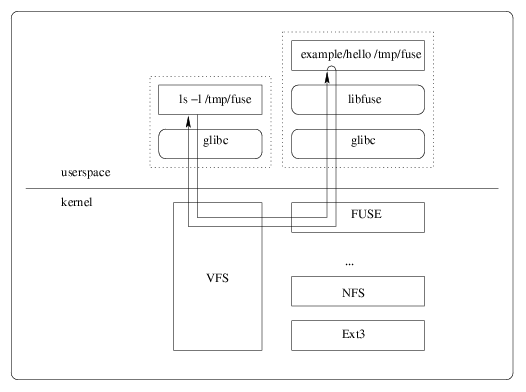
\includegraphics[width=0.9\textwidth]{images/fuse_structure.png}}
\caption{Path of a file system call in the hello world example.}
\label{fig:fuse}
\end{figure}

Figure \ref{fig:fuse} shows the path of a file system call in the provided hello world example file system. We can see the \texttt{FUSE} kernel module acting as a proxy between the \texttt{VFS} system call and the \texttt{example/hello} user space code. A kernel space file system would not need to re-enter user space to compete the system call, hence giving better performance. 

The \texttt{FUSE} library provides a number of function definitions which the user space code implements. These functions are then called when the corresponding file system operation occurs. Some of the important operations are discussed in detail below.\\

\begin{lstlisting}[language=C, caption={\texttt{FUSE} read operation.}, frame=single]
	int read(const char *path, char *buf, size_t size, off_t offset, struct fuse_file_info *fi);
\end{lstlisting}

\noindent
The \texttt{read} function is called when a file system read occurs. It requests that \texttt{size} bytes of the file \texttt{path} starting at offset \texttt{offset} should be written to the buffer \texttt{buf}.

The \texttt{write} function is similar:\\

\begin{lstlisting}[language=C, caption={\texttt{FUSE} write operation.}, frame=single]
	int write(const char *path, const char *buf, size_t size, off_t offset, struct fuse_file_info *fi);
\end{lstlisting}

\noindent
It requests that \texttt{size} bytes from the buffer \texttt{buf} should be written to the file \texttt{path} starting at offset \texttt{offset}.

Similar functions exist for all of the standard file system operations, see appendix section ??? for a full list. 

\subsection{Existing tools}
% worth citing this: http://www.pedramhayati.com/images/docs/survey_of_steganography_and_steganalytic_tools.pdf
The relatively little work on steganography within video is reflected in my search for steganographic programs operating on video files. This section contains an exhaustive list of all the video steganogrphy tools I could find freely\footnote{A further 2 programs exist claiming to embed within video, however these are closed source and not freely available to download. Therefore they have been excluded from this list. (Info Stego, Hiderman)} available on the Internet. A total of 6 tools claimed to provide steganographic embedding functionality within video files. Of these 6, only 3 actually attempt to embed within the video data itself. None of the identified programs allow the user to embed more than one file\footnote{Admittedly you could embed a compressed archive using these tools to effectively allow a directory structure to be embedded.}  and none of them provide any sort of file system interface.

\subsubsection{StegoStick}

\texttt{StegoStick} claims to allow users to ``hide any file into any file''. This statement suggests that the program is simply appending the requested file to the end of the cover object. This suspicion is partly true; based on the file extension, \texttt{StegoStick} splits cover objects into 3 categories: images, media and other. The other category does indeed just append the file to the cover object, whereas the image and media category do attempt to employ steganographic embedding methods. The images category applies to files with extensions \texttt{JPG}, \texttt{GIF} and \texttt{BMP} and uses LSB embedding within \texttt{BMP} files (other image formats are converted to \texttt{BMP} prior to embedding). The media category applies to \texttt{WAV}, \texttt{AVI} and \texttt{MPG} files and assumes each format has a ``header'' of 44+55 bytes\footnote{Listed in the source as ``44 byte header + 54 bytes of extension space''.}. Although this seems to be true for the \texttt{WAV} format, this is not the case for \texttt{AVI} nor \texttt{MPG} files. \texttt{StegoStick} will then use blind LSB embedding within the remaining data. As such, my attempts to use \texttt{StegoStick} to embed within \texttt{AVI} files rendered the resulting video unplayable. % (I haven't actually done this...) 

\subsubsection{StegoMagic}

\texttt{StegoMagic} claims to ``work on all types of files and all size of data'' which again sounds as though it's appending the file to the end of the cover object. This is indeed the case, embedding an image within a video and inspecting the modified file shows that data has just been appended to the end of the video, albeit encrypted. \texttt{StegoMagic} does not specify the encryption algorithm used and the source code is not available to view. Furthermore, the user cannot specify an encryption key to use. Instead, \texttt{StegoMagic} generates a 5 digit number during the embedding process and echos this to the user.  

\subsubsection{TCSteg}

\texttt{TCSteg} is a Python script accompanying a blog post written by Martin Fiedler discussing hiding TrueCrypt volumes within \texttt{MP4} files. The method described embeds the TrueCrypt volume within the MP4 atom \texttt{mdat} and modifies the chunk offset table within the \texttt{moov} atom so that any application playing the video will ignore the embedded data. A nice property of \texttt{TCSteg} is that the resulting video file can be directly mounted by TrueCrypt since it ignores the MP4 header data prior to the embedded volume.\\

\noindent
The above programs all resort to embedding within video files by either appending the embedded data to the end of the video, or inserting the embedded data at some point within the video file. I do not consider this approach to embedding data secure, and it should be a trivial task for any steganalyst to detect the presence of embedded data within the stego objects using a simple hex editor. Therefore, the above stegosystems should be considered broken and definitely not used for the hiding of sensitive data.

\subsubsection{StegoVideo}

\texttt{StegoVideo} is a Virtual Dub filter\footnote{Which is also available in a stand alone executable form.} which allows users to embedded a file within \texttt{AVI} files (supporting multiple compression codecs). I am unsure of the exact steganograhpic embedding algorithm used since the program is closed source, but the website does mention that \texttt{StegoVideo} makes use of error correction codes to allow embedded data to be recovered even after the resulting video has been compressed - although this is understandably dependant on the compression amount. \texttt{StegoVideo} claims to protect the embedded data via the use of a passkey (a 5 digit number), although as with \texttt{StegoMagic}, this is not provided by the user and is instead generated and presented to the user to make a note of.

\subsubsection{OpenPuff}

\texttt{OpenPuff} is a steganographic tool supporting a wide range of formats, including \texttt{3GP}, \texttt{MP4}, \texttt{MPG} and \texttt{VOB}. It allows users to embed a file within a collection of carrier objects and uses 3 user provided passwords to encrypt, scramble and whiten (mixing with a high amount of noise) the provided file. Plausible deniability is also provided via the option to add decoy content. \texttt{OpenPuff} successfully embedded and retrieved a text file within a sample \texttt{MP4} video and I could notice no perceivable impact on video quality. Performance was also good due to multithreading support. However, the embedding capacity is very limited. A hard limit of \SI{256}{\mega\byte} is imposed regardless of the number and size of the carrier objects and I was only able to achieve embedding capacities of around 0.0043\%\footnote{2,600 bytes within a \SI{60}{\mega\byte} video.} even at the maximum capacity setting. This makes \texttt{OpenPuff} impractical for hiding large files - for example, you would need around 770 \SI{60}{\mega\byte} \texttt{MP4} carrier files to embed a standard \SI{2}{\mega\byte} \texttt{JPEG} image.

\subsubsection{Steganosaurus}

\texttt{Steganosaurus} is a cross platform steganograhpic program developed by James Ridgway. It allows users to embed a file within \texttt{MP4} (\texttt{H264}) files via the modification of motion vectors. The input file is encrypted using \texttt{AES} with a user provided pass phrase. Need to test this in Linux.\\

\noindent
The above 3 programs are much more promising from a steganogrphic security point of view and some of them also support multiple video formats. However, all feature the same limitation of only allowing the user to embed one chosen file and the offered embedding capacities are far from practical for use with large files.

This project aims to remedy these issues by providing the user the opportunity to embed an arbitrary number of files within a video via a file system interface and providing high capacity steganographic embedding algorithms offering capacities in excess of 100\%\footnote{This specifically means a file of size n bytes can have more than n bytes hidden inside it.} of the cover object's size\footnote{This is very much a trade off - capacities upwards of 100\% will come at the sacrifice of steganogrphic security. However, this decision is presented to the user rather than decided by the program itself.}. 

\subsection{Requirements Analysis}

After reviewing the necessary background material and investigating current available solutions to the problem of steganography within video, the following collection of requirements were produced. For the project to be considered a success, at least all of the core requirements should be fulfilled.

\subsubsection{Core Requirements}

\texttt{Stegasis} should:

\begin{itemize}
\item Allow users to embed data within video files:
	\begin{itemize}
		\item Several steganographic embedding algorithms should be available.
		\item Each embedding algorithm, $\mathcal{A}$, should satisfy correctness. That is,\\ 
		\begin{center}
			$\forall ~\textbf{c}, \textbf{k}, \textbf{m}. ~Ext_{\mathcal{A}}(Emb_{\mathcal{A}}(\textbf{c}, \textbf{k}, \textbf{m}), \textbf{k}) = \textbf{m}$.
		\end{center}
		\item Steganalysis tools should be developed to test the security of the proposed embedding algorithms.
		\item An optional user provided password should encrypt data prior to embedding.
		\item A capacity option should allow users to specify the percentage of each video frame to embed within.
	\end{itemize}
\item Provide a file system interface:
	\begin{itemize}
		\item The presented logical volume should reside at a user provided mount point.		
		\item Data written to the file system should be embedded on the fly within the chosen video file.
		\item Data accessed from the file system should be retrieved on the fly from within the video.
		\item Standard file system operations such as creating, deleting and moving files should work as expected, and standard Unix tools such as \texttt{cp}, \texttt{mv} and \texttt{rm} should also work as expected.
	\end{itemize}	
\item Support raw uncompressed \texttt{AVI} video:
	\begin{itemize}
		\item Uncompressed \texttt{AVIs} should be natively parsed allowing access to individual pixel data.
	\end{itemize}	
\item Provide performance adequate for normal use:
	\begin{itemize}
		\item Full HD video content should be playable directly from within the presented file system.
	\end{itemize}		
\end{itemize}

\subsubsection{Possible Extensions}

If time constraints allow, the following extension tasks shall also be completed.\\

\noindent
\texttt{Stegasis} should:

\begin{itemize}
\item Support a wide range of video formats:
	\begin{itemize}
		\item Specifically including the popular video format \texttt{MP4}.		
	\end{itemize}
\item Allow directory operations within the file system:
	\begin{itemize}
		\item Creating directories using the \texttt{mkdir} command should work as expected, as should using the \texttt{mv} and \texttt{rm} commands.
		\item Organising files within directories should also work as expected.
	\end{itemize}	
\item Embed also within audio data:
	\begin{itemize}
		\item Data should also be embedded within the (possible) audio stream of the video, therefore increasing the embedding capacity.
	\end{itemize}	
\item Provide plausible deniability:
	\begin{itemize}
		\item A second file system should be (optionally) embedded within the video, mountable with a second passphrase.
		\item The presence of the second, hidden file system should not be detectable.
	\end{itemize}
\item Be evaluated for perceivable video impact using a web application:
	\begin{itemize}
		\item The web application should evaluate the claim ``Embedding has no perceivable impact on video quality.'' by obtaining data from multiple users.
	\end{itemize}		
\end{itemize}

\subsection{Choice of Languages and Tools}

With the above requirements for the final product defined, an appropriate set of languages and tools can be identified.

It is first noted that \texttt{Stegasis} (as developed for this project) will only function on the \texttt{Linux} operating system. That is, there is no requirement for \texttt{Stegasis} to be cross platform.  

The file system is an important aspect of \texttt{Stegasis} and so it is initially decided which approach to take in developing it as this will influence the later choice of an appropriate programming language. As described within section \ref{fs}, it was decided to use the \texttt{FUSE} library to develop the file system component in user space.

We now address the choice of primary programming language for the development of \texttt{Stegasis}.

Several of the core (and extension) requirements strongly suggest a lower level language such as C or C++ rather than a higher level sandboxed language such as Java. For example, the parsing and modification of \texttt{AVI} files lends itself to a language like C since it will involve large amounts of byte level manipulation. Furthermore, the Microsoft file format reference defines the different data structures used within \texttt{AVIs} as C \texttt{structs}. The identified library for implementing the file system aspect - \texttt{FUSE} - is natively a C library (as is the \texttt{libjpeg} library, and libraries provided by \texttt{FFmpeg}). Although wrappers for other languages (including Java) do exist, they seem to be lacking documentation and few are being actively maintained. The requirement that \texttt{Stegasis} should support several steganographic embedding algorithms implores the use of object oriented techniques; defining a \texttt{SteganographicAlgorithm} interface of which each embedding algorithm implements. This suggests C++ over C. The final core requirement, performance, also favours C/C++ over Java\footnote{There have been numerous studies showing that C/C++ code performs better than equivalent Java code.} due to the JVM overheads. 

The reasons above led to the conclusion that C++ should be the primary language used to develop \texttt{Stegasis}.

As discussed in section \ref{ffmpeg}, \texttt{FFmpeg} will be used for the extension task ``\texttt{Stegasis} should support a wide range of video formats'', to allow the decoding and conversion of the many video formats available today, together with library \texttt{libjpeg} discussed in section \ref{jpeg} for the manipulation of \texttt{JPEG} images. 

During the implementation of \texttt{Stegasis}, a number of small steganalysis programs will be developed. These will likely be written in a scripting language such as Python or Matlab since both have extensive library support for mathematical operations.

The extension task ``\texttt{Stegasis} should be evaluated for perceivable video impact using a web application'' will require a website to be developed and hosted for easy access to participants and a database to store the collected user data. \texttt{Node.js} together with the web application framework \texttt{Express} and the database \texttt{MongoDB} was chosen as the development stack for the site. This decision was mainly due to the speed at which you can develop \textit{CRUD} (create, read, update and delete) web applications - essentially what this evaluation site is - and my previous experience with the technologies.


\section{Implementation}

\subsection{Introduction}

The development of \texttt{Stegasis} consisted of the 5 main stages sectioned within this chapter. Firstly, a parser for the \texttt{AVI} file format as discussed in section \ref{avi} was developed allowing direct access to video pixel data. Next, steganographic embedding algorithms were implemented along with corresponding steganalysis tools to test the security of the proposed techniques. The file system was then developed utilising the \texttt{AVI} decoder and steganogrphic algorithms to embed and read data directly into and from video files. Finally, the extension tasks were individually addressed providing support for multiple video formats, directory structures and plausible deniability\footnote{The evaluation site extension task is discussed within the evaluation chapter.}. The testing section provides an overview of the testing processes applied throughout development. 

The actual software development process taken differs from that laid out below; each section was not wholly completed before moving onto the next. Instead, an iterative process was taken across all sections, embracing the modern ``Launch early, iterate often'' methodology. For example, as specified in the project proposal timetable, a simplified version of \texttt{Stegasis} was initially produced only offering one simple embedding algorithm and basic file system functionality. This allowed integration issues to be identified early on, when the code was still very malleable. Once this basic version was working, an iterative approach was then taken to add more functionality and features. For the sake of readability, I have structured the sections below to group together implementation details for each separate concept.

\subsection{AVI Decoder}

Blah AVI blah.

\vfill
\subsection{Steganographic Algorithms}
\subsection{File system}
\subsection{Extensions}
\subsubsection{Supporting multiple video formats}
\label{extffmpeg}
\subsubsection{File system directory structures}
\subsubsection{Plausible deniability}
\subsubsection{Hiding data within audio streams}
\subsection{Testing}

\section{Evaluation}
\subsection{Satisfaction of Requirements}
\subsection{Correctness}
\subsection{Security}
\subsection{Performance}

\section{Conclusions}
\subsection{Future Project Directions}


\begin{thebibliography}{1}

\bibitem{digmedia}
  \emph{Steganography in Digital Media}.
  Jessica Fridrich, 2010.

\end{thebibliography}
% ------------------------------------------------------------------------------
% End document
% ------------------------------------------------------------------------------

\end{document}


